\begin{figure}
    \begin{minipage}{\columnwidth}
        \begin{minipage}{0.45\columnwidth}
        \vfill
        \centering
        \begin{lstlisting}[xleftmargin=1em]
while(ctrlQ.pop() == (*$e_i$*)){
  b = dataQ.pop<1 x idx>();
  e = dataQ.pop<1 x idx>();
  v = dataQ.pop<1 x f32>();
  acc(&out[b,e],v); }
        \end{lstlisting}
        \vfill
        \end{minipage}
        \begin{minipage}{0.54\columnwidth}
        \vfill
        \centering
        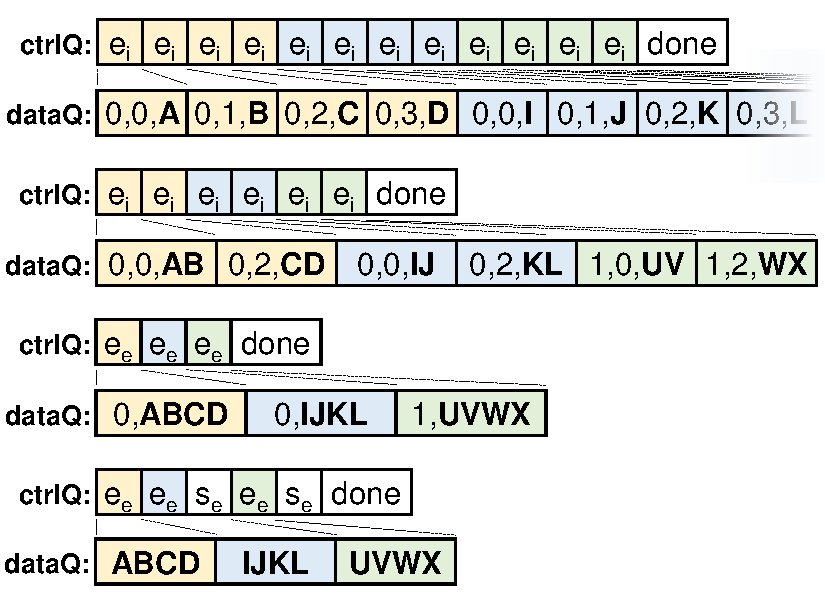
\includegraphics[width=\linewidth, trim={0 3in 0 0},clip]{img_queue_optimizations_impact.pdf}
        \vfill
        \end{minipage}
    \vspace{-0.5em}
    \subcaption{Unoptimized code.}
    \label{fig:ember-dlc-queue-unoptimized-code}
    \end{minipage}
    
    \begin{minipage}{\columnwidth}
        \begin{minipage}{0.45\textwidth}
        \vfill
        \centering
        \begin{lstlisting}[xleftmargin=1em]
while(ctrlQ.pop() == (*$e_i$*)){
  b = dataQ.pop<1 x idx>();
  e = dataQ.pop<1 x idx>();
  v = dataQ.pop<vlen x f32>();
  v_acc(&out[b,e], v);
        \end{lstlisting}
        \vfill
        \end{minipage}
        \begin{minipage}{0.54\textwidth}
        \vfill
        \centering
        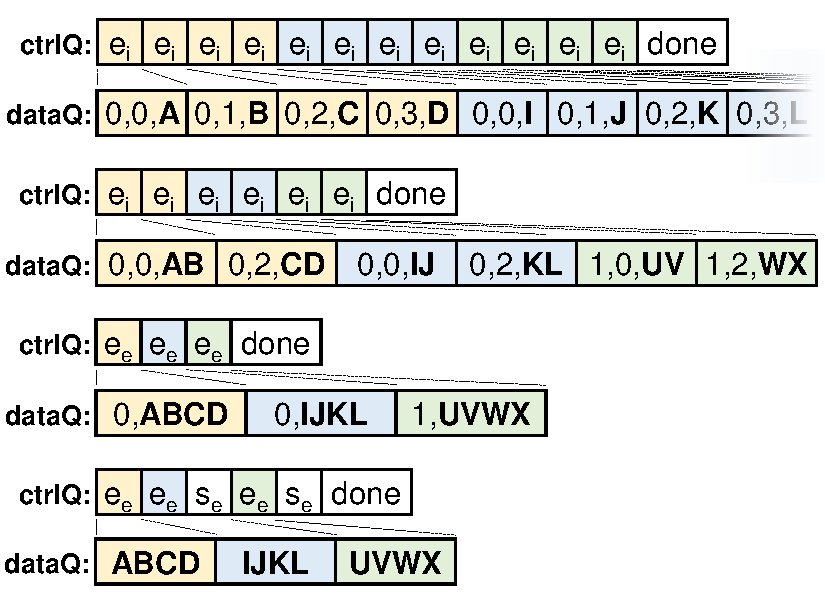
\includegraphics[width=\linewidth, trim={0 2in 0 1in},clip]{img_queue_optimizations_impact.pdf}
        \vfill
        \end{minipage}
    \vspace{-0.5em}
    \subcaption{Vectorized code.}
    \label{fig:ember-dlc-queue-vectorized-code}
    \end{minipage}

    \begin{minipage}{\columnwidth}
        \begin{minipage}{0.45\textwidth}
        \vfill
        \centering
        \begin{lstlisting}[xleftmargin=1em]
while(ctrlQ.pop() == (*$e_e$*)){
  b = dataQ.pop<1 x idx>()
  for(e=0; e<emb_len; e+=vlen){
    v = dataQ.pop<vlen x f32>()
    v_acc(&out[b,e],v) }
        \end{lstlisting}
        \vfill
        \end{minipage}
        \begin{minipage}{0.54\textwidth}
        \vfill
        \centering
        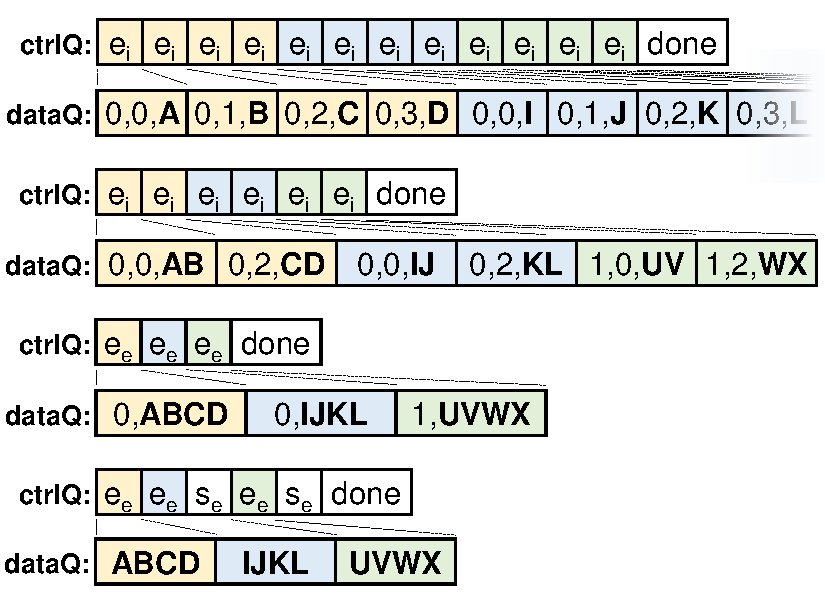
\includegraphics[width=\linewidth, trim={0 1in 0 2in},clip]{img_queue_optimizations_impact.pdf}
        \vfill
        \end{minipage}
    \vspace{-0.5em}
    \subcaption{Buffered code.}
    \label{fig:ember-dlc-queue-buffered-code}
    \end{minipage}

    \begin{minipage}{\columnwidth}
        \begin{minipage}{0.45\textwidth}
        \vfill
        \centering
        \begin{lstlisting}[xleftmargin=1em]
out_ptr = out
while(tkn = ctrlQ.pop() != done){
  if(tkn == (*$e_e$*)){
    for(e=0; e<emb_len; e+=vlen){
      v = dataQ.pop<vlen x f32>()
      v_acc(out_ptr+e, v) }}
  else if(tkn == (*$s_e$*)){
    out_ptr += emb_len }
        \end{lstlisting}
        \vfill
        \end{minipage}
        \begin{minipage}{0.54\textwidth}
        \vfill
        \centering
        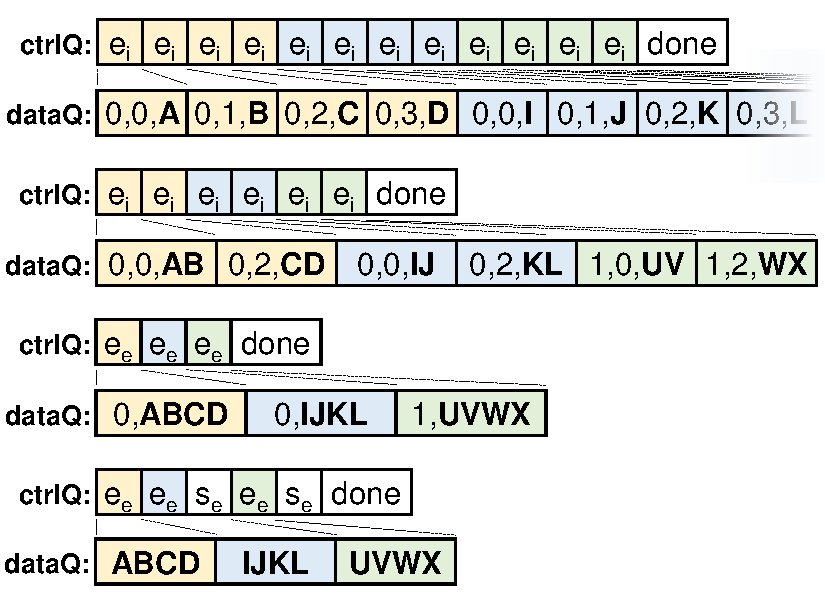
\includegraphics[width=\linewidth, trim={0 0 0 3in},clip]{img_queue_optimizations_impact.pdf}
        \vfill
        \end{minipage}
    \vspace{-0.5em}
    \subcaption{Queue aligned code.}
    \label{fig:ember-dlc-queue-aligned-code}
    \end{minipage}
    
    \caption[Impact of SLC optimizations on DLC queues and compute code.]{Impact of SLC optimizations on DLC EB compute code and output queues. Vectorization widens queued values, buffering groups an entire embedding vector behind one token, and queue alignment removes scalar operands that would otherwise misalign vector data in the queue. Overall, these optimizations reduce queue traffic and improve execute-side vector efficiency.}
    \label{fig:ember-dlc-queue-optimization-impact}
\end{figure}
